\documentclass[a4paper,10pt,titlepage]{article}
% Språk och encodings
\usepackage[swedish,english]{babel}
\usepackage[T1]{fontenc}
\usepackage[utf8]{inputenc}
\usepackage[fixlanguage]{babelbib}
% Images and floats
\usepackage{graphicx}
\usepackage{wrapfig}
\usepackage{float}
% Clear type + Sans-serif font
\usepackage{lmodern}
\renewcommand{\familydefault}{\sfdefault}
% Avancerade tabeller
\usepackage{tabularx}
\usepackage{multirow}
\usepackage{booktabs}
% Matte
\usepackage{amsmath, amsthm, amssymb}
% Algoritmer
\usepackage[ruled,vlined]{algorithm2e}
% Källkod
\usepackage{listings}
\lstset{
	showspaces = false,
	showstringspaces = false,
}
% Inkludera pdf-sidor
\usepackage{pdfpages}
% Länkar
\usepackage{color}
\definecolor{dark-blue}{rgb}{0, 0, 0.6}
\usepackage{hyperref}
\hypersetup{
  colorlinks=true,
  linkcolor=dark-blue,
  urlcolor=dark-blue
}
% Vettiga paragrafer
\setlength{\parindent}{0pt}
\setlength{\parskip}{2ex}

% Kommando för kommandorader
\newcommand{\cmdline}[1]{\mbox{\textbf{\texttt{> #1}}}}

% Kommandon för testfall
\usepackage{testcases}

% Sidhuvud/sidfot
\usepackage{fancyhdr}
\setlength{\headheight}{15pt}
\pagestyle{fancyplain}
\lfoot{Carl-Oscar Erneholm \\ 880422-0872 \\ coer@kth.se}
\rfoot{Martin Nycander \\ 881028-0076 \\ mnyc@kth.se}
\cfoot{Sida \thepage}

% Språk
\selectbiblanguage{swedish}
\selectlanguage{swedish}

% Titel
\title{Laborationsrapport 2 \\ Small-Shell v2.51 för UNIX}
\author{Carl-Oscar Erneholm \and Martin Nycander}
\date{\today}

\begin{document}

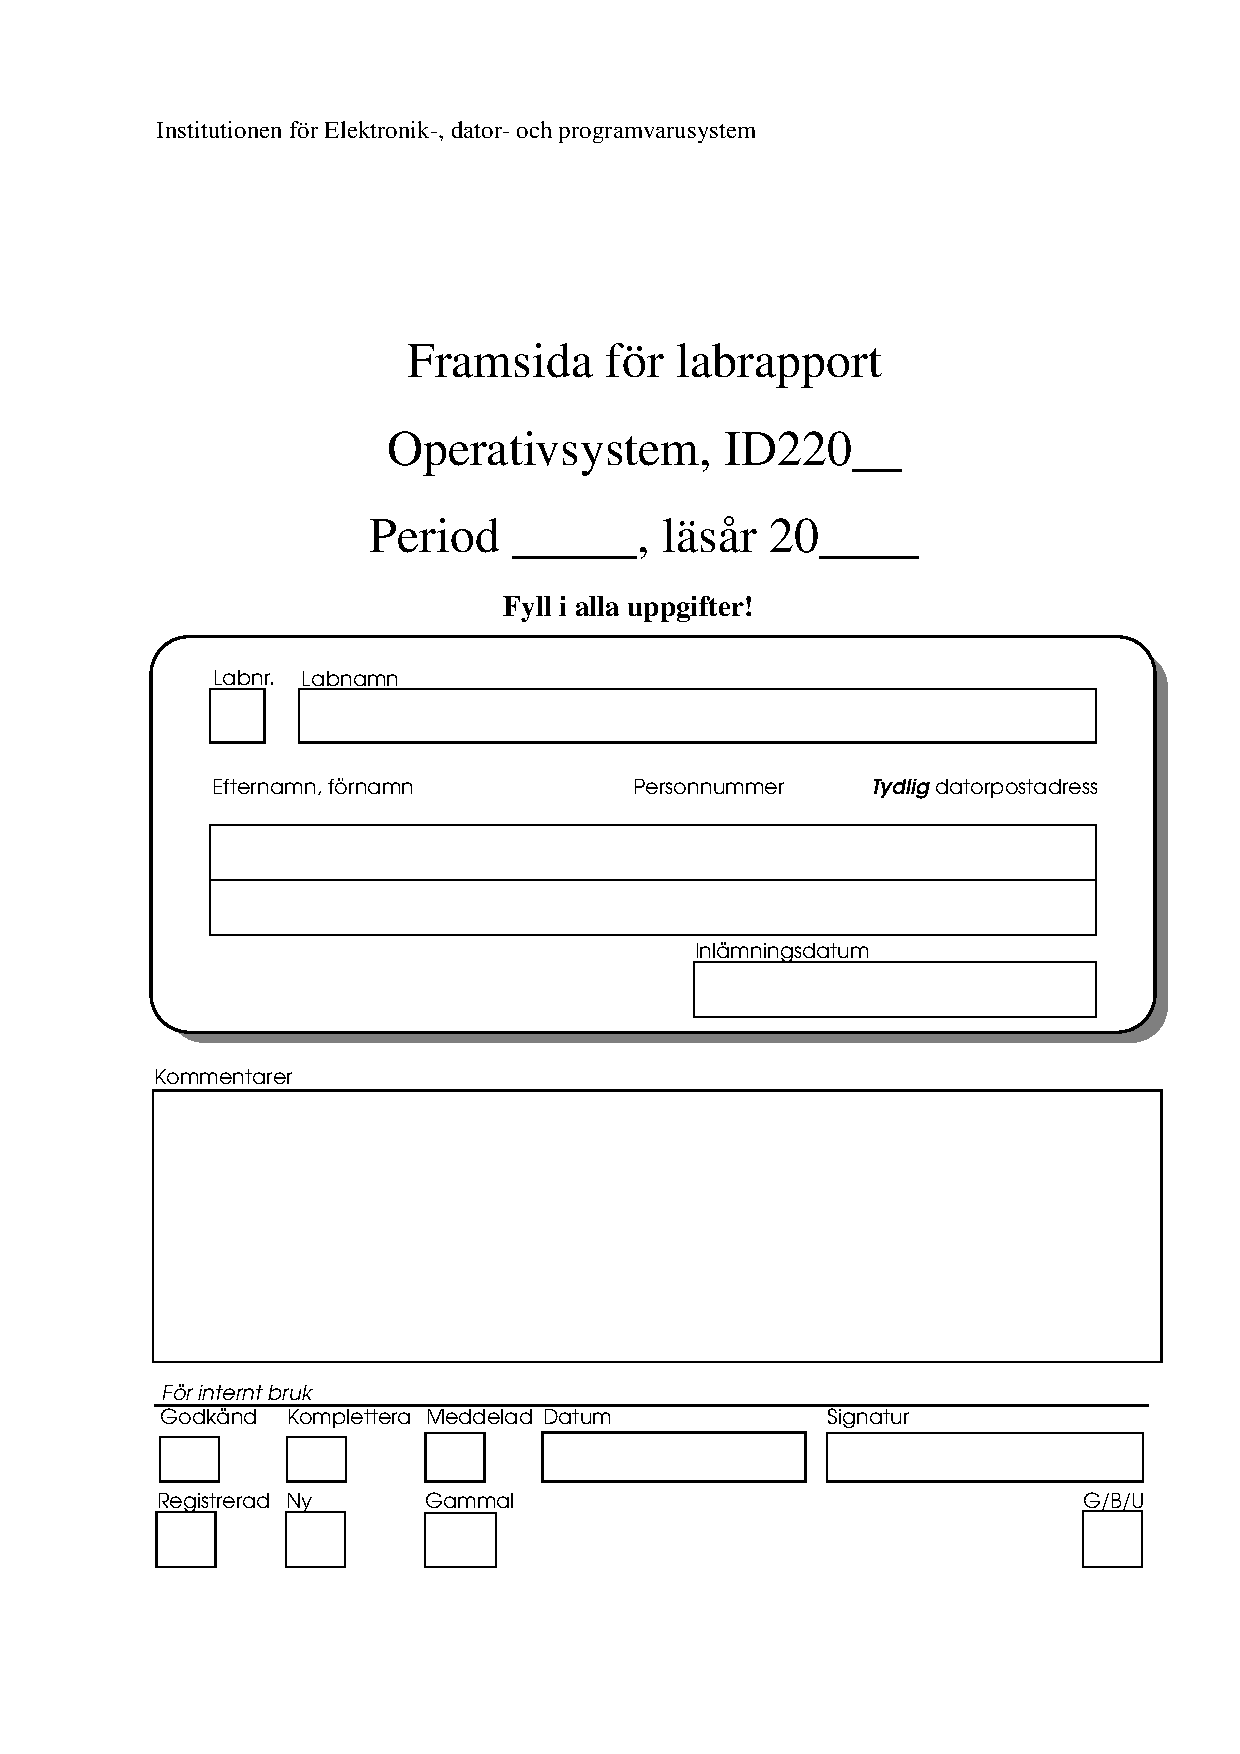
\includepdf[pages=-]{framsida.pdf}

\maketitle

\tableofcontents
\thispagestyle{empty}
\newpage
\setcounter{page}{1}
\section{Problembeskivning}

Uppgiften bestod i att implementera ett minimalt UNIX-skal. Programmet ska såsom
andra skal kunna starta program användaren matar in till dess att användaren
avslutar med kommandot: \verb!exit!. Skalet ska dessutom kunna hantera
förgrunds- och bakgrunds-processer.


\subsection{Förberedelsefrågor}

\begin{enumerate}
	\item[1.] \textbf{\footnotesize Motivera varför det ofta är bra att exekvera kommandon i en separat process.}

    Om ett program som miniShell startar krachar är det enklare att komma
    tillbaka till miniShell prompten.

	\item[2.] \textbf{\footnotesize Vad händer om man inte i kommandotolken exekverar wait() för en barn-process som avslutas?}
	Barn-processen kommer finnas kvar som zombieprocess tills dess att skal
    programmet avslutas.

	\item[3.] \textbf{\footnotesize Hur skall man utläsa SIGSEGV?}

	\item[4.] \textbf{\footnotesize Varför kan man inte blockera SIGKILL?}
    För att man inte ska kunna skapa odödliga processer.

	\item[5.] \textbf{\footnotesize Hur skall man utläsa deklarationen void (*disp)(int))?}
	
    Det är en funktionspekare som pekar på en funktion som returnerar void och
    tar en int som parameter.

	\item[6.] \textbf{\footnotesize Vilket systemanrop använder sigset(3C) troligtvis för att installera en signalhanterare?}
	Förmodligen sigaction.

	\item[7.] \textbf{\footnotesize Hur gör man för att din kommandotolk inte skall termineras då en förgrundsprocess i den termineras med <Ctrl-c>?}
	Vi ignorerar inkommande SIGINT signaler, med hjälp av ett anrop av sigaction.

	\item[8.] \textbf{\footnotesize Studera körningsexemplet nedan och förklara varför man inte har bytt “working directory” till /home/ds/robertr när man avslutat miniShell:et?}
    cd som förmodligen är implementerad med chdir ändrar bara “working
    directory” på den process som anropar den. I det här fallet är det miniShell
    som anropar funktionen och därför ändras bara miniShells “working directory”
    ändringen går därför förlorad när processen dör.

\end{enumerate}

\newpage
\section{Programbeskrivning}

Programmet utvecklades i enlighet med den föreslagna arbetsgången. Vad som hjälpte en hel del var att skapa små program för varje funktion. Med andra ord inte bara \verb!execvp! och \verb!fork! utan även för bakgrundsprocesser och signalhanterare.

Bakgrundsprocesser skapades enkelt genom att inte göra någon låsande \verb!wait! efter \verb!fork!:en, utan istället installera en signalhanterare som kallade på \verb!waitpid! med \verb!WNOHANG!-flaggan så att funktionen returnerar direkt. Alternativet, ``polling'', implementeras genom att köra waitpid i början av loopen som kör nya processer, så att bakgrundsprocesser rensas upp efter att en förgrundsprocess har kört.

Immunitet mot keyboard interrupts (SIGINT) görs genom att en signalhanterare installeras med handlerfunktionen \verb!SIG_IGN!. Standardhanteraren sparas undan för att sedan återinstalleras i nya förgrundsprocesser vilket gör att förgrundsprocesser kan avslutas med \verb!Ctrl+c!, men inte skalprogrammet i sig.

\newpage
\section{Tester}

För att testa funktionaliten av vårat program har vi valt att köra följande kontrollerade tester:

\begin{testcase}{Start av förgrundsprocess}
	\prereq{\begin{checklist}
		\item Kommandotolken är startad.
		\item Programmet \texttt{echo} finns.
	\end{checklist}}
	\actions{
		\cmdline{echo "Test"}
	}
	\result{\begin{checklist}
			\item ``Test'' skrivs ut i kommandotolken.
			\item \texttt{echo} terminerar ordentligt (kontrollera med \cmdline{ps -aux}).
		\end{checklist}}
\end{testcase}

\begin{testcase}{Tomma strängen}
	\prereq{Kommandotolken är startad.}
	\actions{Ge ingen input, tryck bara enter.}
	\result{Kommandotolken kraschar inte.}
\end{testcase}

\begin{testcase}{Start av bakgrundsprocess}
	\prereq{\begin{checklist}
		\item Kommandotolken är startad.
		\item Programmet \texttt{sleep} finns.
		\item Programmet \texttt{echo} finns.
	\end{checklist}}
	\actions{\begin{actionlist}
		\item \cmdline{sleep 10\&}
		\item \cmdline{echo "Test"}
	\end{actionlist}
	}
	\result{\begin{checklist}
			\item Man behöver inte vänta 10 sekunder innan man får köra \cmdline{echo "Test"}
			\item ``Test'' skrivs ut i kommandotolken.
			\item Programmen terminerar ordentligt (kontrollera med \cmdline{ps -aux}).
		\end{checklist}}
\end{testcase}

\begin{testcase}{Bakgrundsprocesser och förgrundsprocesser}
	\prereq{\begin{checklist}
		\item Kommandotolken är startad.
		\item Programmet \texttt{sleep} finns.
	\end{checklist}}
	\actions{\begin{actionlist}
		\item \cmdline{sleep 5\&}
		\item \cmdline{sleep 10}
	\end{actionlist}
	}
	\result{\begin{checklist}
			\item Programmen terminerar i rätt ordning (först \cmdline{sleep \&}, sedan \cmdline{sleep 10}).
			\item Programmen terminerar ordentligt (kontrollera med \cmdline{ps -aux}).
		\end{checklist}}
\end{testcase}

\begin{testcase}{Avslutning med ``exit''}
	\prereq{Kommandotolken är startad.}
	\actions{\cmdline{exit}}
	\result{\begin{checklist}
		\item Kommandotolken avslutas.
		\item Inga zombie-processer finns kvar (kontrollera med \cmdline{ps -aux}).
	\end{checklist}}
\end{testcase}

\begin{testcase}{Byte av arbetskatalog}
	\prereq{\begin{checklist}
		\item Kommandotolken är startad.
		\item Environmentvariabeln \texttt{HOME} är satt till ett känt värde.
	\end{checklist}}
	\actions{\begin{actionlist}
		\item Exekvera ``\cmdline{cd}''
		\item Exekvera ``\cmdline{pwd}'' och notera resultatet (1).
		\item Exekvera ``\cmdline{cd /etc}''
		\item Exekvera ``\cmdline{pwd}'' och notera resultatet (2).
		\item Exekvera ``\cmdline{cd .}''
		\item Exekvera ``\cmdline{pwd}'' och notera resultatet (3).
		\item Exekvera ``\cmdline{cd /åäö404}''
		\item Exekvera ``\cmdline{pwd}'' och notera resultatet (4).
		\item Exekvera ``\cmdline{cd.}''
		\item Exekvera ``\cmdline{pwd}'' och notera resultatet (5).
	\end{actionlist}}
	\result{\begin{checklist}
		\item Resultat 1, 4 och 5 borde vara samma som värdet på \texttt{HOME}-variabeln.
		\item Resultat 2 och 3 borde vara ``/etc''.
	\end{checklist}}
\end{testcase}

\begin{testcase}{Informationsutskrifter}
	\prereq{\begin{checklist}
		\item Kommandotolken är startad.
		\item Programmet \texttt{sleep} finns.
	\end{checklist}}
	\actions{\cmdline{sleep 2}}
	\result{
		Följande information skrivs ut:
		\begin{checklist}
			\item Processid
			\item Att det är en förgrundsprocess.
			\item Att processen skapades och terminerades.
			\item Statistik över hur lång tid kommandot tog att genomföra.
		\end{checklist}
	}
\end{testcase}

\begin{testcase}{Terminering med Ctrl+c}
	\prereq{\begin{checklist}
		\item Kommandotolken är startad.
		\item Programmet \texttt{sleep} finns.
	\end{checklist}}
	\actions{\begin{actionlist}
		\item \cmdline{sleep 20}
		\item Avsluta exekveringen med \texttt{Ctrl+c} innan programmet avslutar sig själv.
	\end{actionlist}}
	\result{\begin{checklist}
		\item \texttt{sleep} avslutas (kontrollera med ps -aux).
		\item Kommandotolken avslutas \textbf{inte}.
	\end{checklist}}
\end{testcase}

\newpage
\section{Resultat}

Körning av ovanstående standardiserade testfall gav följande resultat.

\begin{testresults}{\today}
\end{testresults}

\newpage
\section{Labbutvärdering}

\newpage
\section{Källkod}

\lstset{tabsize=2}
\footnotesize{\lstinputlisting[language=C]{../program/minishell.c}}

\end{document}
